\section{Implementation}
\subsection{Simulated Network}

\subsubsection{Controller}

\subsubsection{Actuator}

\subsubsection{Sensor}

\subsubsection{Internet Cloud}

\subsubsection{Factory Access Point}

\subsubsection{Factory Bridge}

\subsection{MATLAB Simulation}
  Our MATLAB 

\subsubsection{Tennessee Eastman}
  We buit a custom simplified Tennesee Eastman model in MATLAB.  
  This was based off of a preexisting FORTRAN model, but was
  reimplemented in MATLAB for ease of use and reduced complexity 
  \citation{Ricker}.  Our model contains variable vectors, an
  input vector, a state vector, and an output vector. Then by 
  using the equations provided in Ricker\citation{Ricker}, the
  simulation simply takes in the input vector from OMNeT++, and
  outputs the output vector, which includes the sensor data, to
  OMNeT++ via the MATLAB bridge.

\subsection{C++ to MATLAB Bridge}

\begin{figure*}
        \centering
		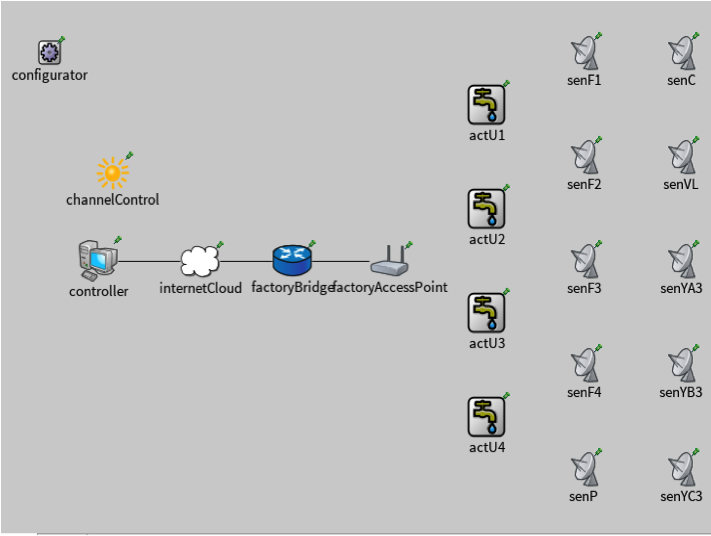
\includegraphics[width=0.8\textwidth]{figs/network.png}
        \caption{Network Diagram.}
        \label{fig:system}        
\end{figure*}
